\chapter{Example Outputs of a Single Segmentation Round}\label{app:segmentedOutput}

This appendix is provided as example to assist in visualizing the different outputs generated during segmentation.  Figure~\ref{fig:segmentationGroundTruthImages} shows the two ground-truth images that were input into the Mixed-Bag Solver for this example.  As explained in Section~\ref{sec:Segmentation}, pieces from these images are assembled as if they had come from a single puzzle;  Figure~\ref{fig:segmentationAssemblerOutput} is the assembler output for the first round of segmentation.  Figure~\ref{fig:segmentationRepresentation} shows the segments (they are colored to make them easier to identify) identified in the assembler output.  For each segment, the pieces that are further away from an open location are lighter in color while those closer to a boundary are darker.  Although not strictly a part of segmentation, the stitching piece(s) that would have resulted from each segment (assuming it exceeded the minimum size) are marked with white crosses as a reference.

Figure~\ref{fig:bestBuddiesAssemblerOutput} is the best buddy visualization of the assembler output.  Note that the right and left sides of image~(a) have stripes of best buddies that extend only in the horizontal direction.  All of the pieces in these stripes are articulation points.  As such, they were removed from the main segment in the center of the image as described in Section~\ref{sec:articulationPoints}.

\begin{figure}
\centering
  \begin{tabular}{ >{\centering\arraybackslash}m{0.47\textwidth} >{\centering\arraybackslash}m{0.47\textwidth} }

	\fbox{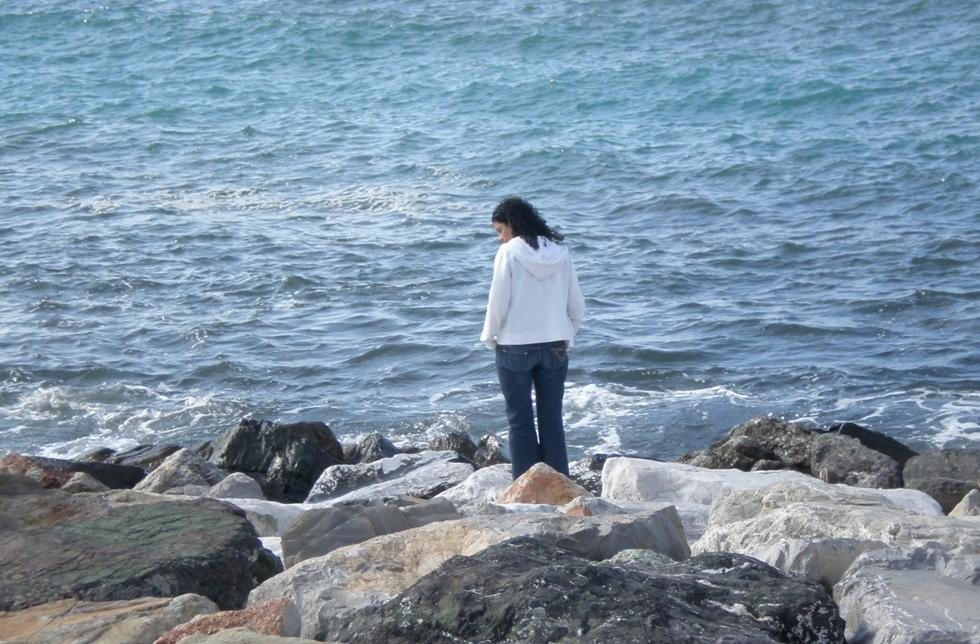
\includegraphics[scale=0.16]{./images/segmentation/pomeranz_805_8.jpg}} & \fbox{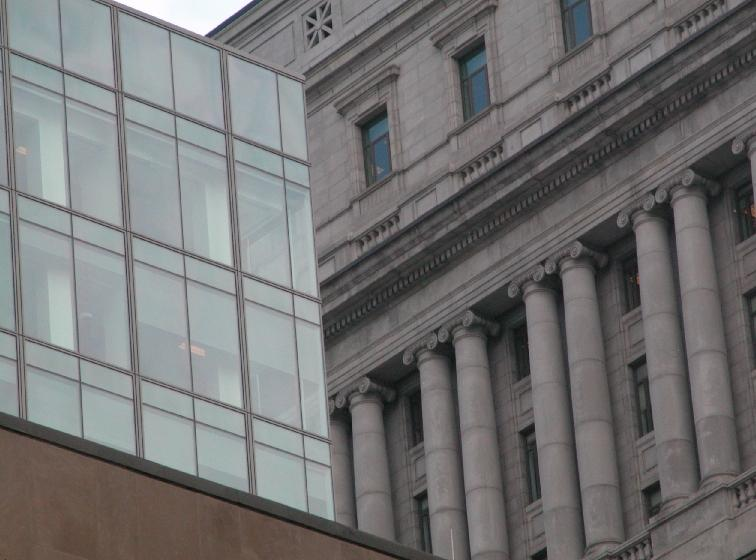
\includegraphics[scale=0.16]{./images/segmentation/mcgill_540_20.jpg}} \\~\\
	Image~(a) \textendash { }805~Pieces~\cite{pomeranzBenchmarkImages} \ & Image~(b) \textendash { }540~Pieces~\cite{mcgillImageDatabase}\\~\\
  \end{tabular}

\caption{Ground-Truth Images Used in the Segmentation Example}
\label{fig:segmentationGroundTruthImages}
\end{figure}

\begin{figure}
\centering
  \begin{tabular}{ >{\centering\arraybackslash}m{0.9\textwidth} }
	\fbox{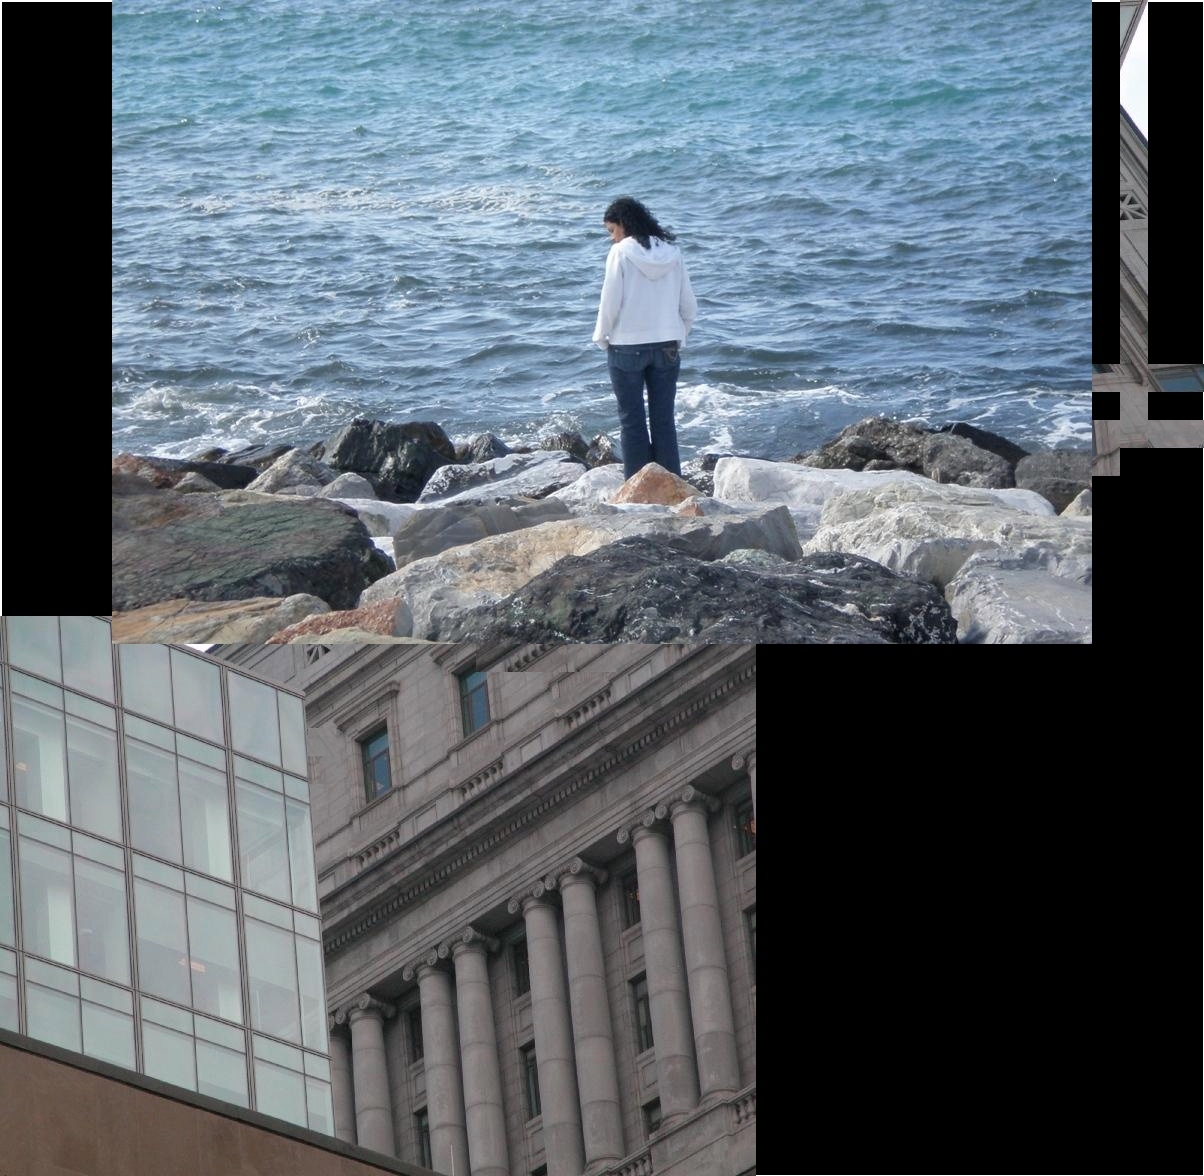
\includegraphics[scale=0.16]{./images/segmentation/assembler_single_puzzle_output.jpg}} \\~\\
  \end{tabular}

\caption{Assembler Output of a Single Puzzle after the First Segmentation Round}
\label{fig:segmentationAssemblerOutput}
\end{figure}

\begin{figure}
\centering
  \begin{tabular}{ >{\centering\arraybackslash}m{0.95\textwidth} }
	\fbox{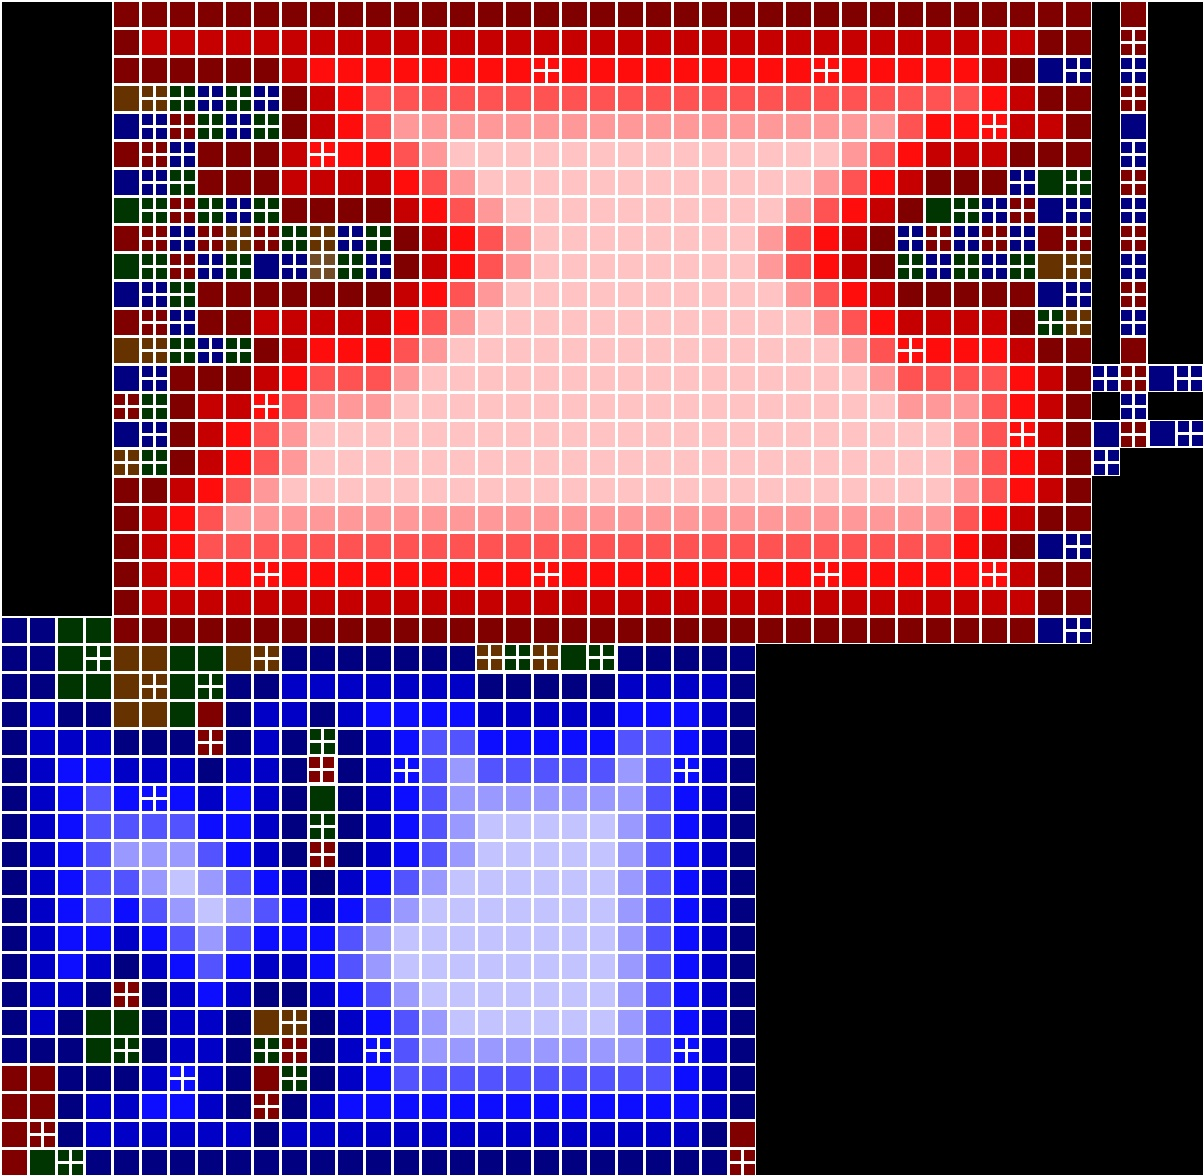
\includegraphics[scale=0.16]{./images/segmentation/segmentation_assembler_output.jpg}} \\~\\
  \end{tabular}
\caption{Segmentation of the Assembler Output with Marking of the Articulation Points and the Lightness of Piece Coloring Dependent on the Distance to the Nearest Open Location}
\label{fig:segmentationRepresentation}
\end{figure}

\begin{figure}
\centering
  \begin{tabular}{ >{\centering\arraybackslash}m{0.95\textwidth} }
	\fbox{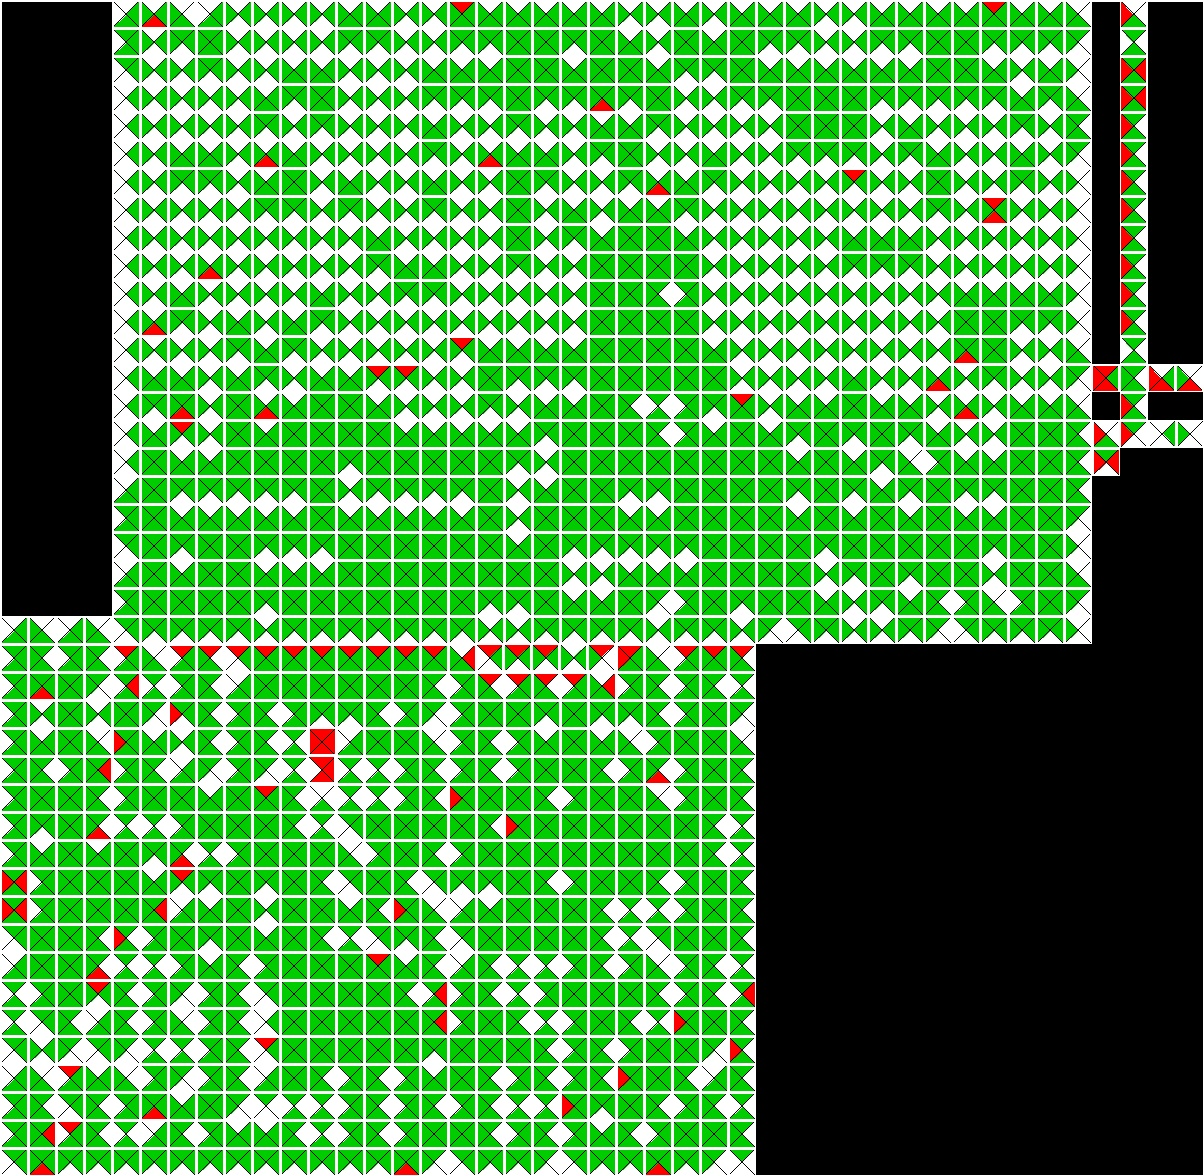
\includegraphics[scale=0.16]{./images/segmentation/best_buddy_assembler_output.jpg}} \\~\\
  \end{tabular}
\caption{Best Buddy Visualization of the Assembler Output}
\label{fig:bestBuddiesAssemblerOutput}
\end{figure}
